\documentclass[11pt]{beamer}
\usetheme{Warsaw}
\usepackage[utf8]{inputenc}
\usepackage[british,UKenglish,USenglish,english,american]{babel}
\usepackage[T1]{fontenc}
\usepackage{amsmath}
\usepackage{amsfonts}
\usepackage{amssymb}
\usepackage{graphicx}

\addtobeamertemplate{footline}{\insertframenumber/\inserttotalframenumber}

\author{Arnaud De Bruecker, MediVisu}
\title{MediVisu}

\setbeamercovered{transparent}
\logo{
\includegraphics[width=0.5cm]{esi.png}}
\institute{HEB - ESI} 
\date{2015 - June}

\begin{document}

\begin{frame}
\titlepage
\end{frame}

\begin{frame}
\frametitle{Table of contents}
\tableofcontents
\end{frame}

\section{Context}

\begin{frame}
\frametitle{Context}
\begin{itemize}[<+->]
\item[•] Many manufacturers with proprietary solutions;
\begin{itemize}[<+->]
\item[•] Incompatibilities between each others;
\item[•] Very expensive;
\item[•] Not suitable to patients.
\end{itemize}
\item[•] There are free software alternatives but
\begin{itemize}[<+->]
\item[•] Often exclusive to one platform;
\item[•] Uncertified (FDA);
\item[•] Non user-friendly.
\end{itemize}
\end{itemize}
\end{frame}

\section{Inspiration}

\subsection{Osirix}

\begin{frame}
\frametitle{Osirix}

\includegraphics[scale=0.17]{Osirix.jpg}
\begin{itemize}[<+->]
\item[•] Developped by a doctor, Antoine Rosset
\item[•] Appreciated by the professionals
\item[•] Restricted to Mac OS X
\item[•] Doesn't read proprietary DICOM fields
\item[•] GPL license
\end{itemize}
\end{frame}

\subsection{Orthanc}

\begin{frame}
\frametitle{Orthanc}

\includegraphics[scale=0.15]{Orthanc.png}
\begin{itemize}[<+->]
\item[•] Belgian project
\item[•] Created by Sébastien Jodogne
\item[•] 2014 Free Software Award winner
\item[•] DICOM server for medical imaging
\item[•] GPL license
\end{itemize}
\end{frame}

%\subsection{3DSlicer}
%
%\begin{frame}
%\frametitle{3DSlicer}
%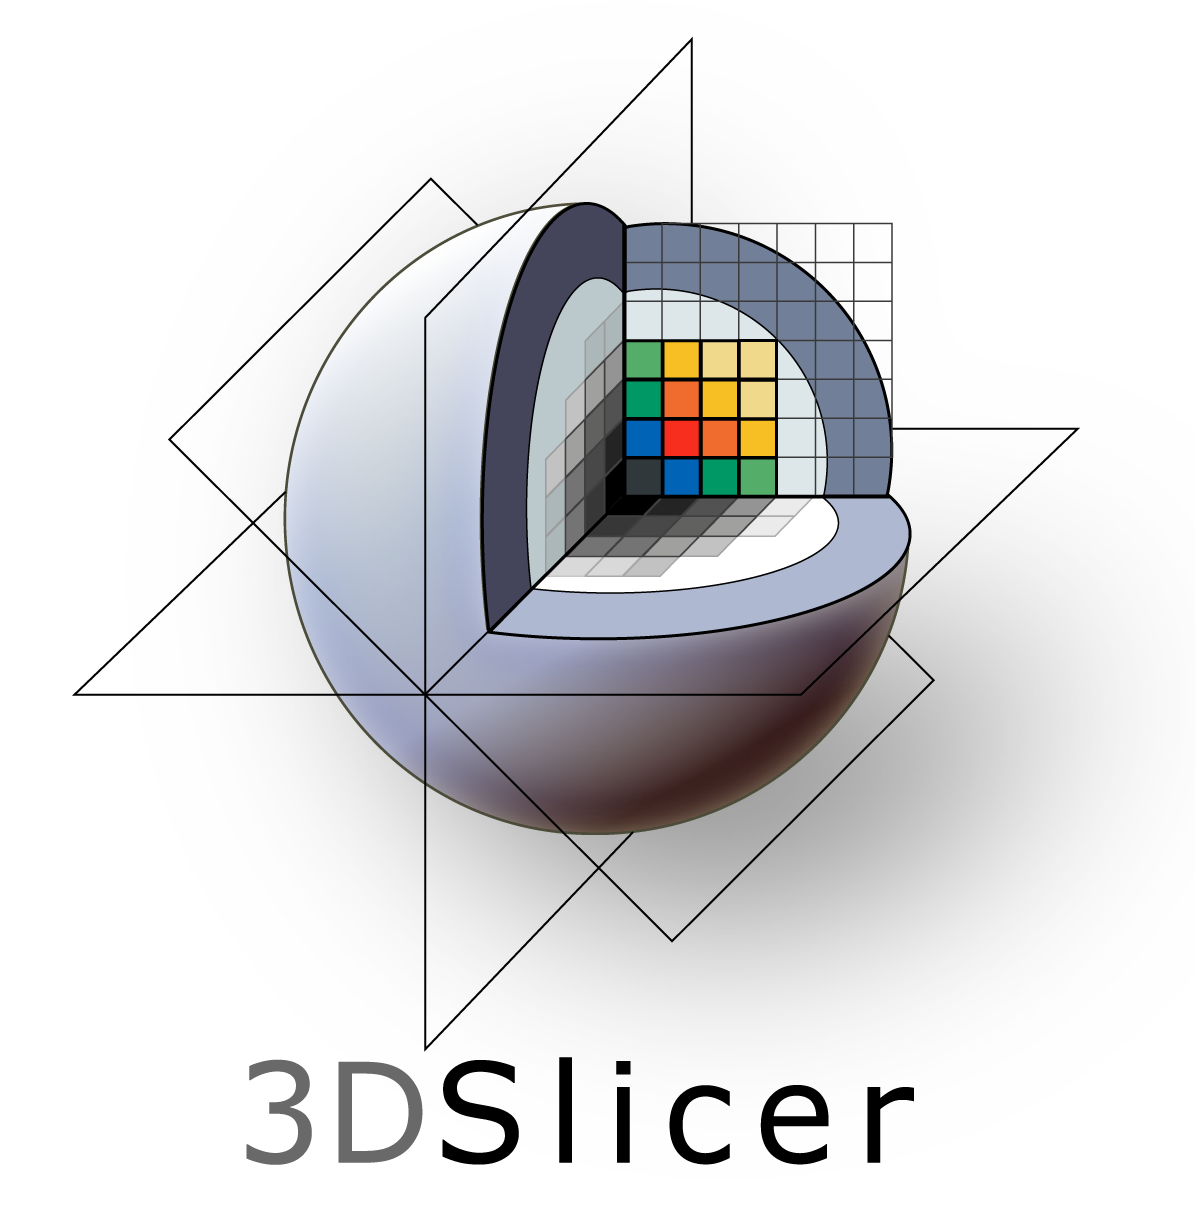
\includegraphics[scale=0.06]{Slicer.png}
%\begin{itemize}[<+->]
%\item[•] Mature free project (is being developped since 1998)
%\item[•] Huge developper community
%\item[•] Medical imaging analysis, tailored for researchers
%\item[•] BSD license
%\end{itemize}
%\end{frame}

%\section{What is a Free Software?}
%
%\subsection{Four Freedoms}
%
%\begin{frame}
%\frametitle{Four Freedoms}
%Participatory development method based on these four freedoms :
%\begin{itemize}[<+->]
%\item[•] The freedom to run the program for any purpose.
%\item[•] The freedom to study how the program works, and change it to make it do what you wish.
%\item[•] The freedom to redistribute copies so you can help your neighbor.
%\item[•] The freedom to improve the program, and release your improvements (and modified versions in general) to the public, so that the whole community benefits.
%\end{itemize}
%\end{frame}
%
%\subsection{Advantages}
%
%\begin{frame}
%\frametitle{Advantages}
%\begin{itemize}[<+->]
%\item[•] Open project
%\begin{itemize}
%\item[•] Exponential workforce with ressources and skills sharing
%\item[•] Potentially guaranteed maintenance
%\end{itemize}
%\item [] Unfortunately, there is often a lack of professional user assistance.
%\end{itemize}
%\end{frame}

%\section{Free but not free}

\section{Commercial ambitions}

\begin{frame}
\frametitle{Commercial ambitions}
\begin{itemize}[<+->]
\item[•] Support and services for users
\begin{itemize}[<+->]
\item[•] Payment is based on a priority system
\end{itemize}
\item[•] Trainings
\item[•] Certification
\end{itemize}
\end{frame}

\section{Software ambitions}

\begin{frame}
\frametitle{MediVisu}
MediVisu ambitions to be:
\begin{itemize}[<+->]
\item[•] Able to read all DICOM fields
\item[•] Free and will remain as such: a foundation will manage rigths
\item[•] Lightweight and easy to apprehend (user-friendly)
\item[•] Customizable with profiles management system and presets for each specialization
\item[•] Multi-platform (Windows, Mac OS X, GnuLinux at least)
\item[•] Certified for medical diagnosis (FDA approved \& CE labeled)
\item[•] Focused on the user experience
\item[•] AGPL license
\end{itemize}
\end{frame}

\section{Challenges}

\begin{frame}
\frametitle{Challenges}
\begin{quote}
\begin{itemize}[<+->]
\item[•] How to break in the industry of medical imaging ?
\item[•] What are the good practices in the creation of a new compagny?
\end{itemize}
\end{quote}
\end{frame}

\begin{frame}
  \frametitle{Links}
    
  \begin{thebibliography}{10}
        
  \beamertemplatearticlebibitems
 
%  \bibitem{3DSlicer}
%  	3DSlicer
%    \newblock Steve Pieper
%    \newblock Available at {\tt http://www.slicer.org}
%
%   \beamertemplatearticlebibitems
 
  \bibitem{Osirix}
  	Osirix
    \newblock Antoine Rosset
    \newblock Available at {\tt http://www.osirix-viewer.com}
    
    \beamertemplatearticlebibitems
 
  \bibitem{Orthanc}
  	Orthanc
    \newblock Sébastien Jodogne
    \newblock Available at {\tt http://www.orthanc-server.com}
    
    \bibitem{MediVisu}
    MediVisu
    \newblock Contact us at {\tt medivisu-dev@pettiaux.be}
 
  \end{thebibliography}
\end{frame}

\end{document}